\chapter{The AK-MCS algorithm}
\label{ch:5}
Crude Monte Carlo Simluations are easy to implement and robust in dealing with 
reliability problems. However, they require the evaluation of the expensive performance
function a considerable amount of times. AK-MCS\sidenote{stands for Active learning method combining Kriging and
Monte Carlo Simulation and is described in
\citep{Echard2011}}, that  and must be seen as a modification of the traditional MCS,
aims to overcome this downside making use Gaussian Processes
Regressions and a learning function to optimize the number of calls of the performance function
on a Monte Carlo simulation.
\section{Preliminaries}
\subsection{Gaussian Identity of conditional distributions}
The joint probability density of the multivariate Gaussian distribution is given by:
\begin{equation}
  p(\bm{x}|\bm{m},\bm{\Sigma}) = (2\pi)^{D/2}|\bm{\Sigma}|^{-1/2}\exp{\left(-\frac{1}{2}(\bm{x}-\bm{m})^{T}\bm{\Sigma}^{-1}(\bm{x}-\bm{m})\right)}
\end{equation}
where $\bm{x}$ is a vector of length $D$, $\bm{m}$ is the mean vector, and $\bm{\Sigma}$ is the covariance matrix, which is symmetric and positive definite. To say that $\bm{x}$ follows a Gaussian distribution with mean  $\bm{m}$ and covariance $\bm{\Sigma}$ we write $\bm{x} \sim \mathcal{N}(\bm{m}, \bm{\Sigma})$. \\

Let $\bm{x}$ and $\bm{y}$ be jointly Gaussian random vectors
\begin{equation}
  \begin{bmatrix}
    \bm{x} \\ \bm{y}
  \end{bmatrix}
  \sim \mathcal{N}\left(
    \begin{bmatrix}
    \bm{\mu_x} \\ \bm{\mu_y}
    \end{bmatrix} , \begin{bmatrix}
      \bm{A} & \bm{C} \\ \bm{C}^T & \bm{B}
    \end{bmatrix} \right)
\end{equation}

then the conditional distribution of $\bm{x}$ given $\bm{y}$ is:
\begin{equation}
  \bm{x}|\bm{y} \sim \mathcal{N}\left(\bm{\mu_x} + \bm{C} \bm{B}^{-1}(\bm{y}-\bm{\mu_y}), \; \bm{A} - \bm{C}\bm{B}^{-1}\bm{C}^T \right)
\end{equation}
The proof of this fact can be detailed in \citep{Bishop}, section 3.1.

\subsection{Gaussian Processes}
A Gaussian process, is a collection of random variables, any finite number of which have a joint Gaussian distribution. It is completely specified by its mean function and covariance function.

\begin{equation}
  f(\bm{x}) \sim \mathcal{GP}(m(\bm{x}), k(\bm{x}, \bm{x'}))
\end{equation}

\begin{equation}
  \begin{bmatrix}
    \bm{y} \\ \bm{\mathrm{f}}_*
  \end{bmatrix}
  \sim \mathcal{N}\left(
  \bm{0}, \begin{bmatrix}
      \bm{K}+\sigma_n^2 \bm{I} & \bm{K}_* \\ \bm{K}_*^T & \bm{K}
    \end{bmatrix} \right)
\end{equation}
\section{Step-by-step of the method}
\begin{enumerate}
    \item \textbf{Generation of a Monte Carlo population in the design space.}
    According to the involved random variables, this population named $S$ of $n_{MC}$ points 
    is generated.
    \item \textbf{Definition of the initial design of experiments (DoE).} The initial
    DoE consists of a random selection of $N_1$ points of $S$. It is preferred to be
    small, adding at each iteration only the point that improves the metamodel
    the most. We will be using a dozen points as suggested in \citep{Echard2011}.
    \item \textbf{Computation of the Kriging model.} The Kriging regressor is trained
    with the performance function $G$ evaluated on the initial DoE. A model with an
    squared-exponential kernel is used.
    \item \textbf{Prediction by Kriging and estimation of the probability of failure.}
    Predictions of the performance function over the Monte Carlo population, $\widehat{G}(x_i)$
    for $i = 1, ..., n_{MC}$ are made with the previously trained Kriging model. 
    Then, the estimated probability of failure $\widehat{p_f}$ is obtained by calculating the ratio
    of the points $x_i \in S$ such that $\widehat{G}(x_i) \leq 0$, i.e.:
    \begin{equation}
        \widehat{p_f} = \frac{n_{\widehat{G}(x_i) \leq 0}}{n_{MC}}
    \end{equation}
    \item \textbf{Identification of the best next point in $S$ to be evaluated on the
    performance function.} At this stage, the learning function is computed for each
    point of $S$ to determine the next point that should be added to the DoE to
    improve the most the metamodel.
    \item \textbf{Evaluation of the stopping condition.} The stopping condition
    associated to the learning function is evaluated for the point selected in the
    previous stage. If the criterion is met, we skip to Stage 8. Otherwise, we
    continue with Stage 7.
    \item \textbf{Update of the design of experiments.}
    The point identified at stage 5 is added to the current DoE, such that $N_{i+1} = N_i + 1$.
    Then, the method goes back to Stage 3.
    \item \textbf{Computation of the coefficient of variation of the probability of
    failure} If the stopping condition is satisfied, the metamodel is said to be
    accurate enough on the sign of the performance function on $S$. Subsequently,
    it is checked if $S$ is large enough to obtain a low coefficient of variation
    on the estimation of $p_f$. If the coefficient of variation is lesser than
    $5\%$, AK-MCS stops and the last estimation of the probability of failure is
    considered as the result. In other case, it continue to Stage 9.
    \item \textbf{Update of the population.} $S$ is increased with other $n_{MC}$ points from the
    design space generated in the same way that in Stage 1, and proceed back to stage 3.
\end{enumerate} 

\section{Learning Functions}
The learning functions are used to decide the next point of the population to be
included in the DoE. In order to do that, they give a score to each $x_i$ of $S$
according to the value $\widehat{G}(x_i)$ and by its variance $\sigma^2_{\widehat{G}}(x_i)$
given by the Kriging regressor. Every learning function comes along with a learning criterion
and with a stopping condition on the obtained scores.

\subsection{Expected feasibility function (EFF)}
It is defined as
\begin{align}
    EFF(x)= \paren{\widehat{G}(x) - a}& \paren{2 \Phi (C) - \Phi (C^+) - \Phi (C^-)} \nonumber\\
- \sigma_{\widehat{G}}(x) & \paren{2 \phi (C) - \phi (C^+) - \phi (C^-)} \\
+ \epsilon & \paren{\Phi (C^+) + \Phi (C^)-}\nonumber
\end{align}
where
\begin{align*}
    C =& \frac{a-\widehat{G}(x)}{\sigma_{\widehat{G}}(x)} \\
    C^+ =& \frac{(a + \epsilon)-\widehat{G}(x)}{\sigma_{\widehat{G}}(x)} \\
    C^- =& \frac{(a - \epsilon)-\widehat{G}(x)}{\sigma_{\widehat{G}}(x)}
\end{align*}
and $\Phi$ is the standard normal cumulative distribution and $\phi$ the standard
normal density distribution. \\

Proposed in \citep{Bichon2008}. It provides an indication of how well the true value
of $\widehat{G}(x)$ is expected to satisfy the equality $G(x) = a$. In AK-MCS we have
$a = 0$ and $\epsilon = 2 \sigma_{\widehat{G}}(x)$. The learning criterion of $EFF(x)$
is the maximum value, so the best next point to add to DoE is $x^* \in S$ such that
$EFF(x^*) =\text{max}(EFF(x))$. The stopping condition is $EFF(x^*) \leq 0.001$.

\subsection{Learning function U}
\begin{equation}
    U(x) = \frac{\left\lvert \widehat{G}(x)\right\rvert }{\sigma_{\widehat{G}}(x)}
\end{equation}
Proposed in \citep{Echard2011}. Considering that in MCS only the sign of the performance
function is important, this function selects as the next best point of $S$ to be added
to the DoE the one that has the higher potential risk of crossing the separator 
$ \widehat{G}(x) = 0$. Then, the best next point to add to the DoE is $x^* \in S$ such that
$U(x^*) =\text{min}(U(x))$. The stopping condition is $U(x^*) \geq 2$.

\subsection{Learning function H}
\begin{equation}
\begin{split}  
    H(x) =  \left\lvert \ln{\paren{\sqrt{2\pi}\sigma_{\widehat{G}}(x) + \frac{1}
    {2}}} \bracket{\Phi \paren{\frac{D^-}{\sigma_{\widehat{G}}(x)}} -
    \Phi \paren{\frac{-D^+}{\sigma_{\widehat{G}}(x)}}}\right. \\ 
    \left. - \bracket{\frac{D^-}{2}\phi \paren{\frac{D^-}{\sigma_{\widehat{G}}(x)}}
    + \frac{D^+}{2} \phi \paren{\frac{-D^+}{\sigma_{\widehat{G}}(x)}}} \right\rvert
\end{split}
\end{equation}
where 
\begin{align*}
    D^+ =& 2\sigma_{\widehat{G}}(x) + \widehat{G}(x) \\
    D^- =& 2\sigma_{\widehat{G}}(x) - \widehat{G}(x)
\end{align*}

Proposed in \citep{Lv2015}. This function is based on the information entrophy theory and 
it measures the uncertainty of $\widehat{G}(x)$. The best next point to add to the DoE is
$x^* \in S$ such that $H(x^*) =\text{max}(H(x))$. It will be used the same stopping
condition that is chosen in \citep{Lv2015}, it is $H(x^*) \leq 0.5$.

\section{Examples}
In this section some examples are presented. They consist of the statement of the
design space and the performance function. Results of each problem are presented in
tables that contains the number of calls to the performance function $N_{call}$,
the estimated probability of failure $\widehat{p_f}$, the coefficient of variation
for the Monte Carlo method, and the relative error of each method compared to the
probability obtained with the Monte Carlo method.
\subsection{Example 1}
The first example is a simple problem with just one variable, that follows a normal distribution
with mean $0$ and standard deviation $2$, and the performance function considered is \ref{eq:ex1}.

\begin{equation}\label{eq:ex1}
    G(\pmb{x}) = \sin{x}
\end{equation}
The problem is solved only with the learning function $U$, and the metamodel is
initialized with just $5$ points in the initial DoE.


\begin{figure}[h!]
    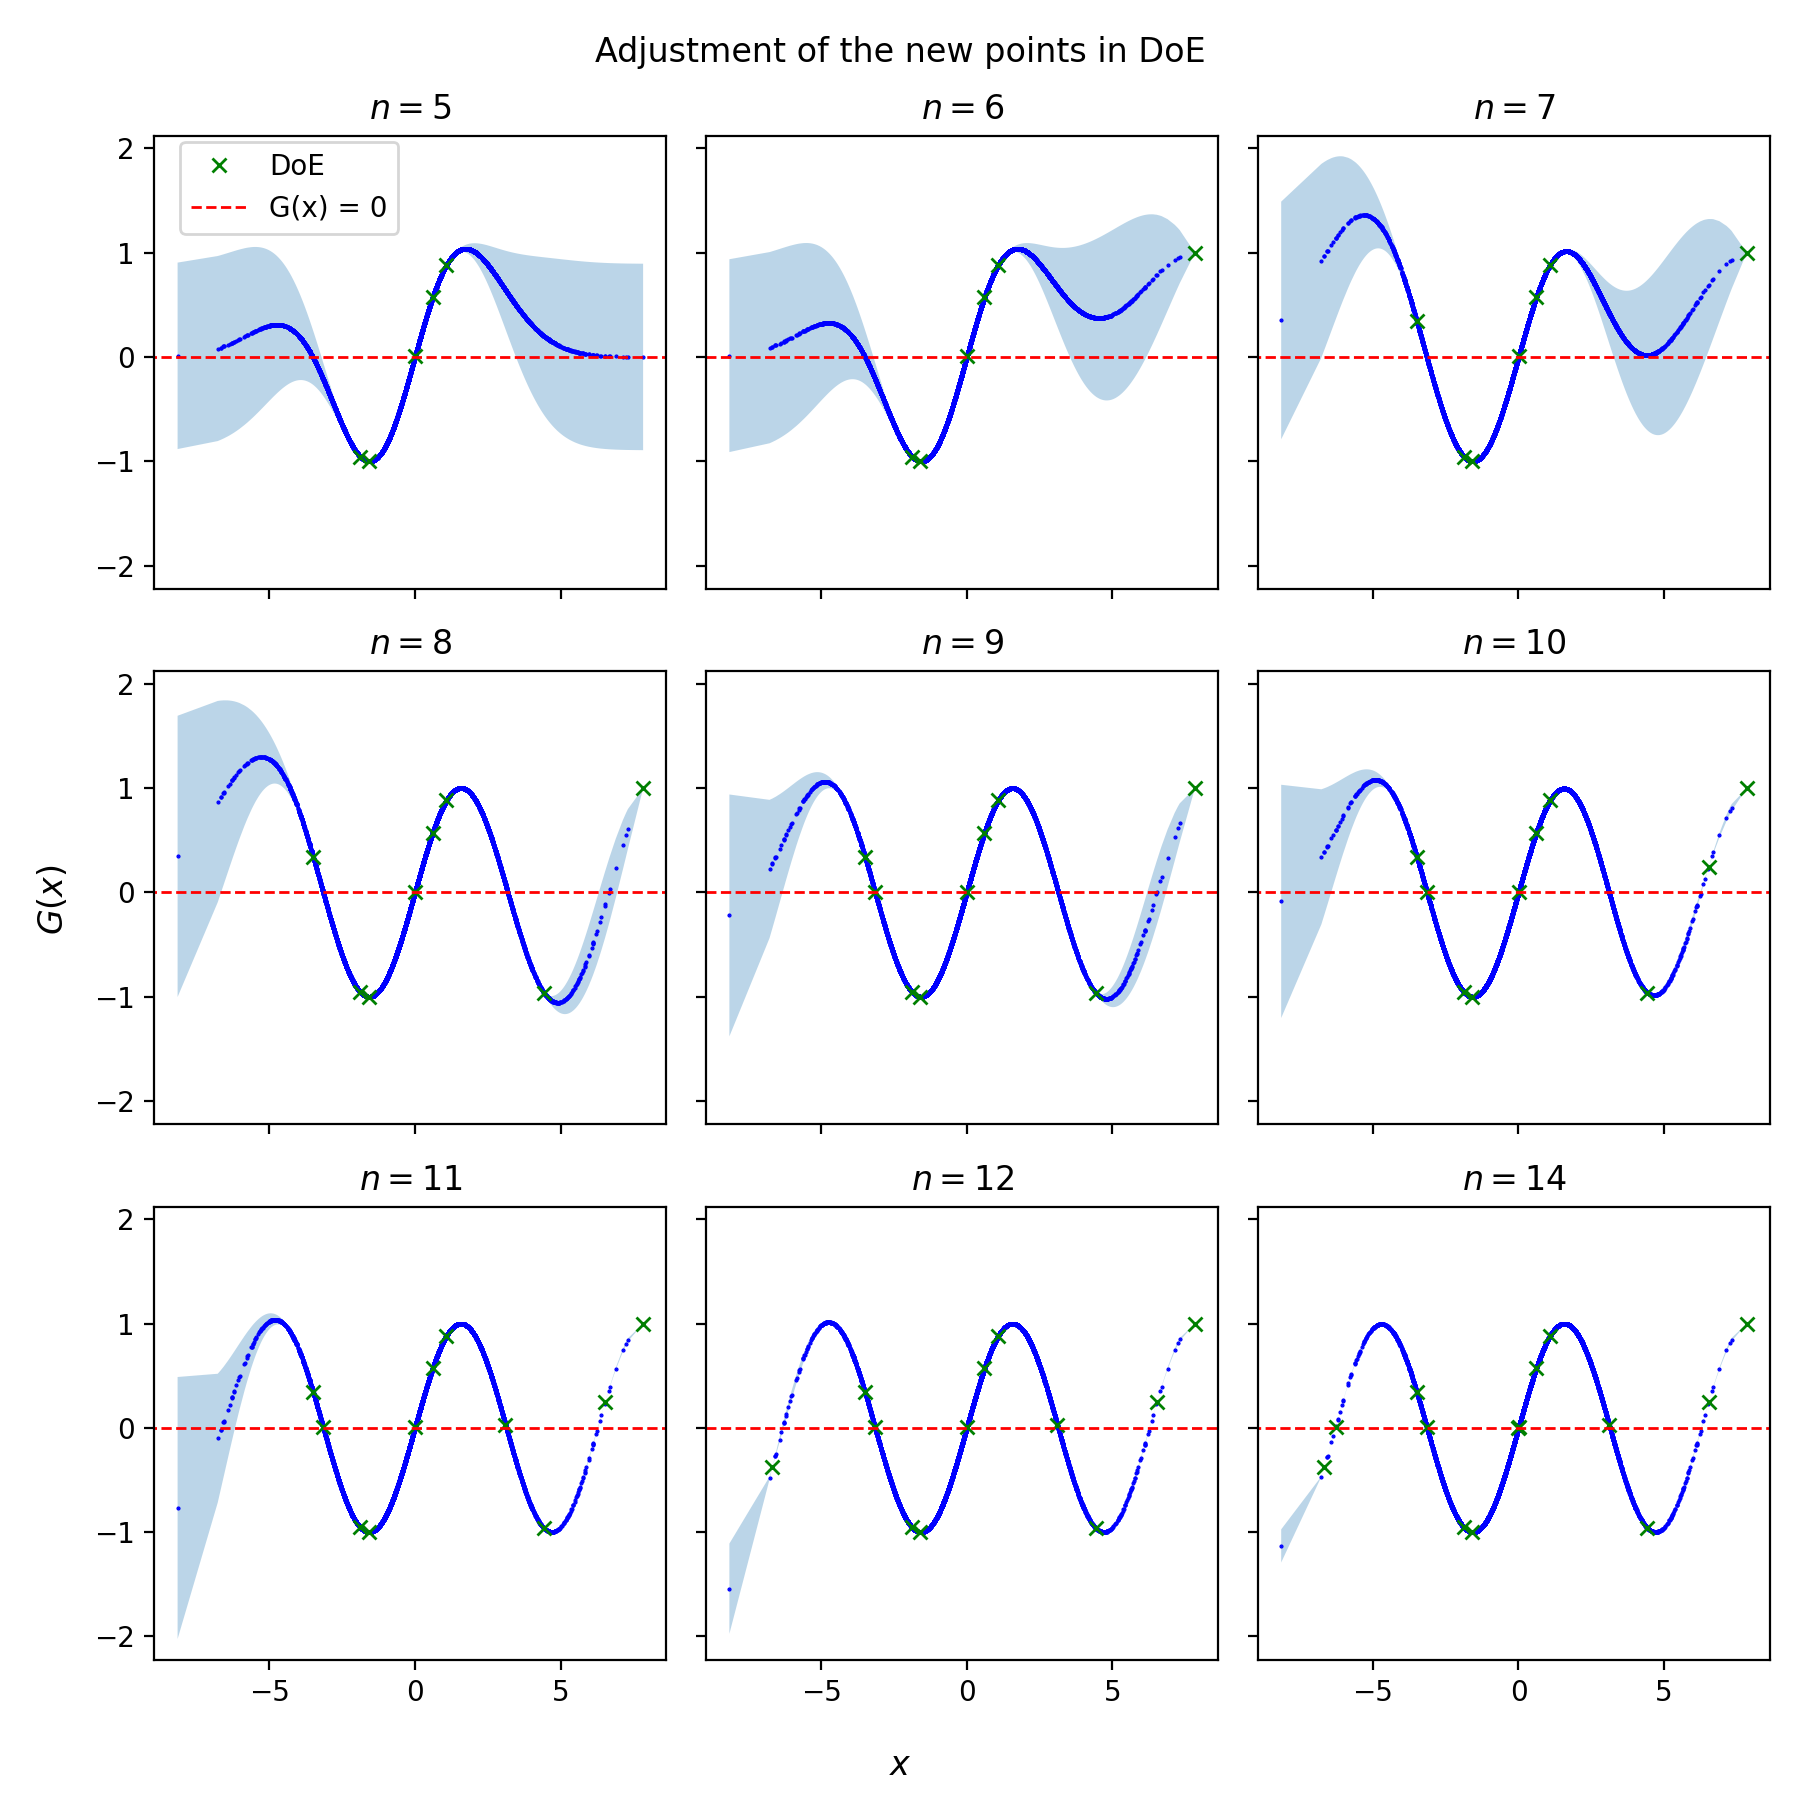
\includegraphics{1d_exa_1d.png}
    \caption{Example 1. Prediction and standard deviation obtained with $n$ points
    in the DoE.}
    \label{fig:ex1}
\end{figure}

\begin{table}[h]
  \footnotesize%
  \begin{center}
  \begin{tabular}{lclcc}
  \toprule
  Method & $N_{call}$  & $\widehat{p_f}$ $(\text{C.O.V}_{\widehat{p_f}})$ &$\epsilon_{\widehat{p_f}}(\%)$  \\
  \midrule
  Monte Carlo   & \num[round-precision=1,round-mode=figures]{10000} & \num{0.4944}($1.01\%$) & - \\
  AK-MCS+U & $14$ & \num{0.4944} & $0$ \\
  \bottomrule
  \end{tabular}
  \end{center}
  \caption{Results of example 1}
  \label{tab:res_ex1}
\end{table}

In figure \ref{fig:ex1} it can be seen how the algorithm selects the next point to
be added to the DoE such that it reduces the most the variance near to the limit 
$G(\pmb{x}) = 0$. Even though there is still some considerable variance in some regions,
it stops at $N = 14$ because this uncertainty is away from the limit, so it is
unlikely to affect the estimation of the probability of failure.
In fact, the results in table \ref{tab:res_ex1} reveal that a very accurate estimation
is obtained.

\subsection{Example 2}
In the second place there is a series system with four branches that is worked in 
\citep{Echard2011}. Both random variables
are standard normal distributed. The performance function is:
\begin{equation}
    G(x_1, x_2) = \text{min}
    \left\lbrace
    \begin{array}{c@{}l}
      3 + 0.1(x_1-x_2)^2 - \frac{(x_1+x_2)}{\sqrt{2}}; \\
      3 + 0.1(x_1-x_2)^2 + \frac{(x_1+x_2)}{\sqrt{2}}; \\
      (x_1-x_2) + \frac{4}{\sqrt{2}}; \\
      (x_2-x_1) + \frac{4}{\sqrt{2}}
    \end{array}
    \right\rbrace
  \end{equation}
with $k$ taking two different values: $6$ and $7$.

From the results on tables \ref{tab:res_ex2} and \ref{tab:res_ex2_2} we can see
that the learning function U obtained the most accurate estimations of $\widehat{p_f}$,
being exactly the same of the MCS. In the case $k=6$, the other two functions performed
well, they only failed at clasifying one point. In the other one, with $k=7$, EFF made some
misclassifications, but the learning function H, although calling the performance function
less times, had an error of $30\%$. \\

\begin{table}[h]
    \footnotesize
    \begin{center}
    \begin{tabular}{lclc}
    \toprule
    Method & $N_{call}$  & $\widehat{p_f}$ $(\text{C.O.V}_{\widehat{p_f}})$ &$\epsilon_{\widehat{p_f}}(\%)$  \\
    \midrule
    Monte Carlo   & \num[round-precision=1,round-mode=figures]{1000000} & \num{0.004433}($1.5\%$) & - \\
    AK-MCS+U & $126$ & \num{0.004433} & $0$ \\
    AK-MCS+EFF & $123$ & \num{0.004432} & $0.02$ \\
    AK-MCS+H & $113$ & \num{0.004434} & $0.02$ \\
    \bottomrule
    \end{tabular}
    \end{center}
    \caption{Results of example 2 with $k=6$}
    \label{tab:res_ex2}
\end{table}

\begin{table}[h]
    \footnotesize
    \begin{center}
    \begin{tabular}{lclc}
    \toprule
    Method & $N_{call}$  & $\widehat{p_f}$ $(\text{C.O.V}_{\widehat{p_f}})$ &$\epsilon_{\widehat{p_f}}(\%)$  \\
    \midrule
    Monte Carlo   & \num[round-precision=1,round-mode=figures]{1000000} & \num{0.002161}($2.15\%$) & - \\
    AK-MCS+U & $103$ & \num{0.002161} & $0$ \\
    AK-MCS+EFF & $107$ & \num{0.002156} & $0.23$ \\
    AK-MCS+H & $65$ & \num{0.0015} & $30.59$ \\
    \bottomrule
    \end{tabular}
    \end{center}
    \caption{Results of example 2 with $k=7$}
    \label{tab:res_ex2_2}
\end{table}

In the figure \ref{fig:ex2_mc} the actual distribution of the two classes in the
MC population is displayed, while in the figure \ref{fig:ex2_iteru} there is the
distribution predicted by AK-MCS+U at several stages. Additionally, figure \ref{fig:ex2_iteru}
give some insights about the update of the DoE, showing how the selected points tend to
come from near the limit $G(\pmb{x}) = 0$. \\

\begin{figure}[h]
    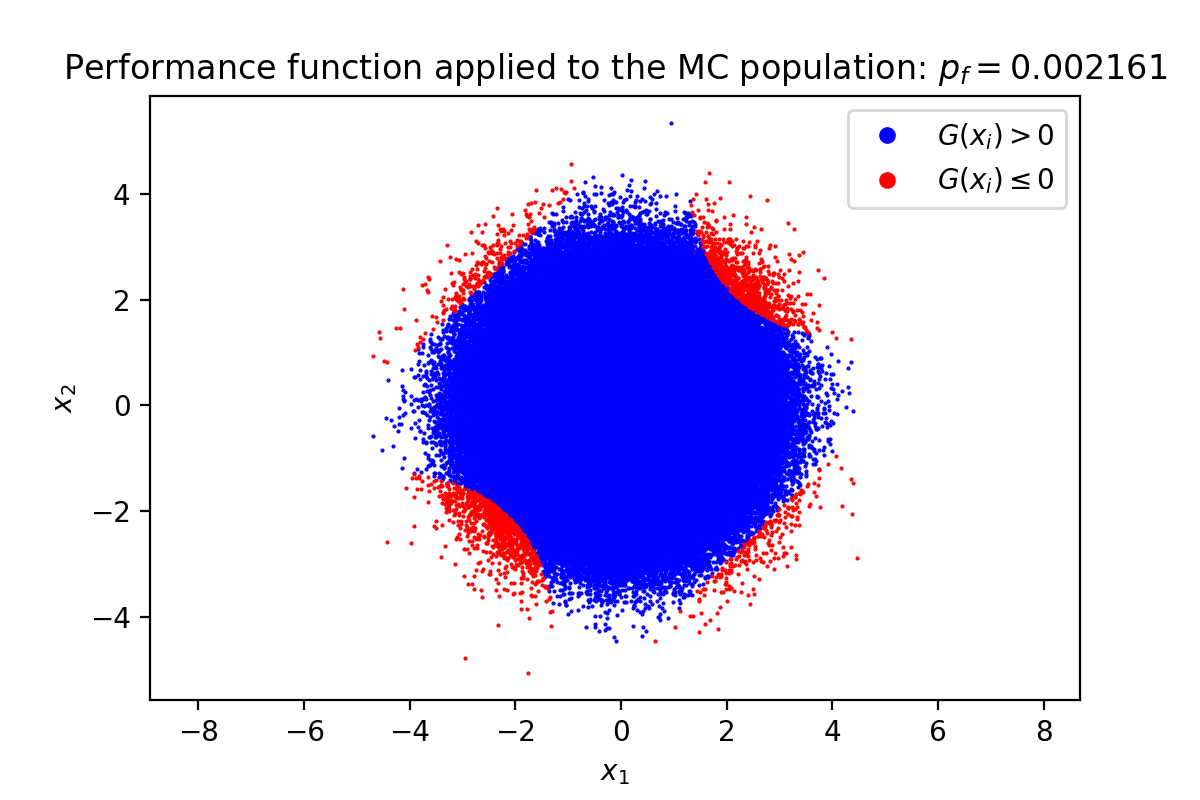
\includegraphics[width=0.8\linewidth]{mc_ex_2D_k7.png}
    \caption{Example 2 with $k=7$. Evaluation of the performance function on the MC population.}
    \label{fig:ex2_mc}
\end{figure}

\begin{figure*}[h]
    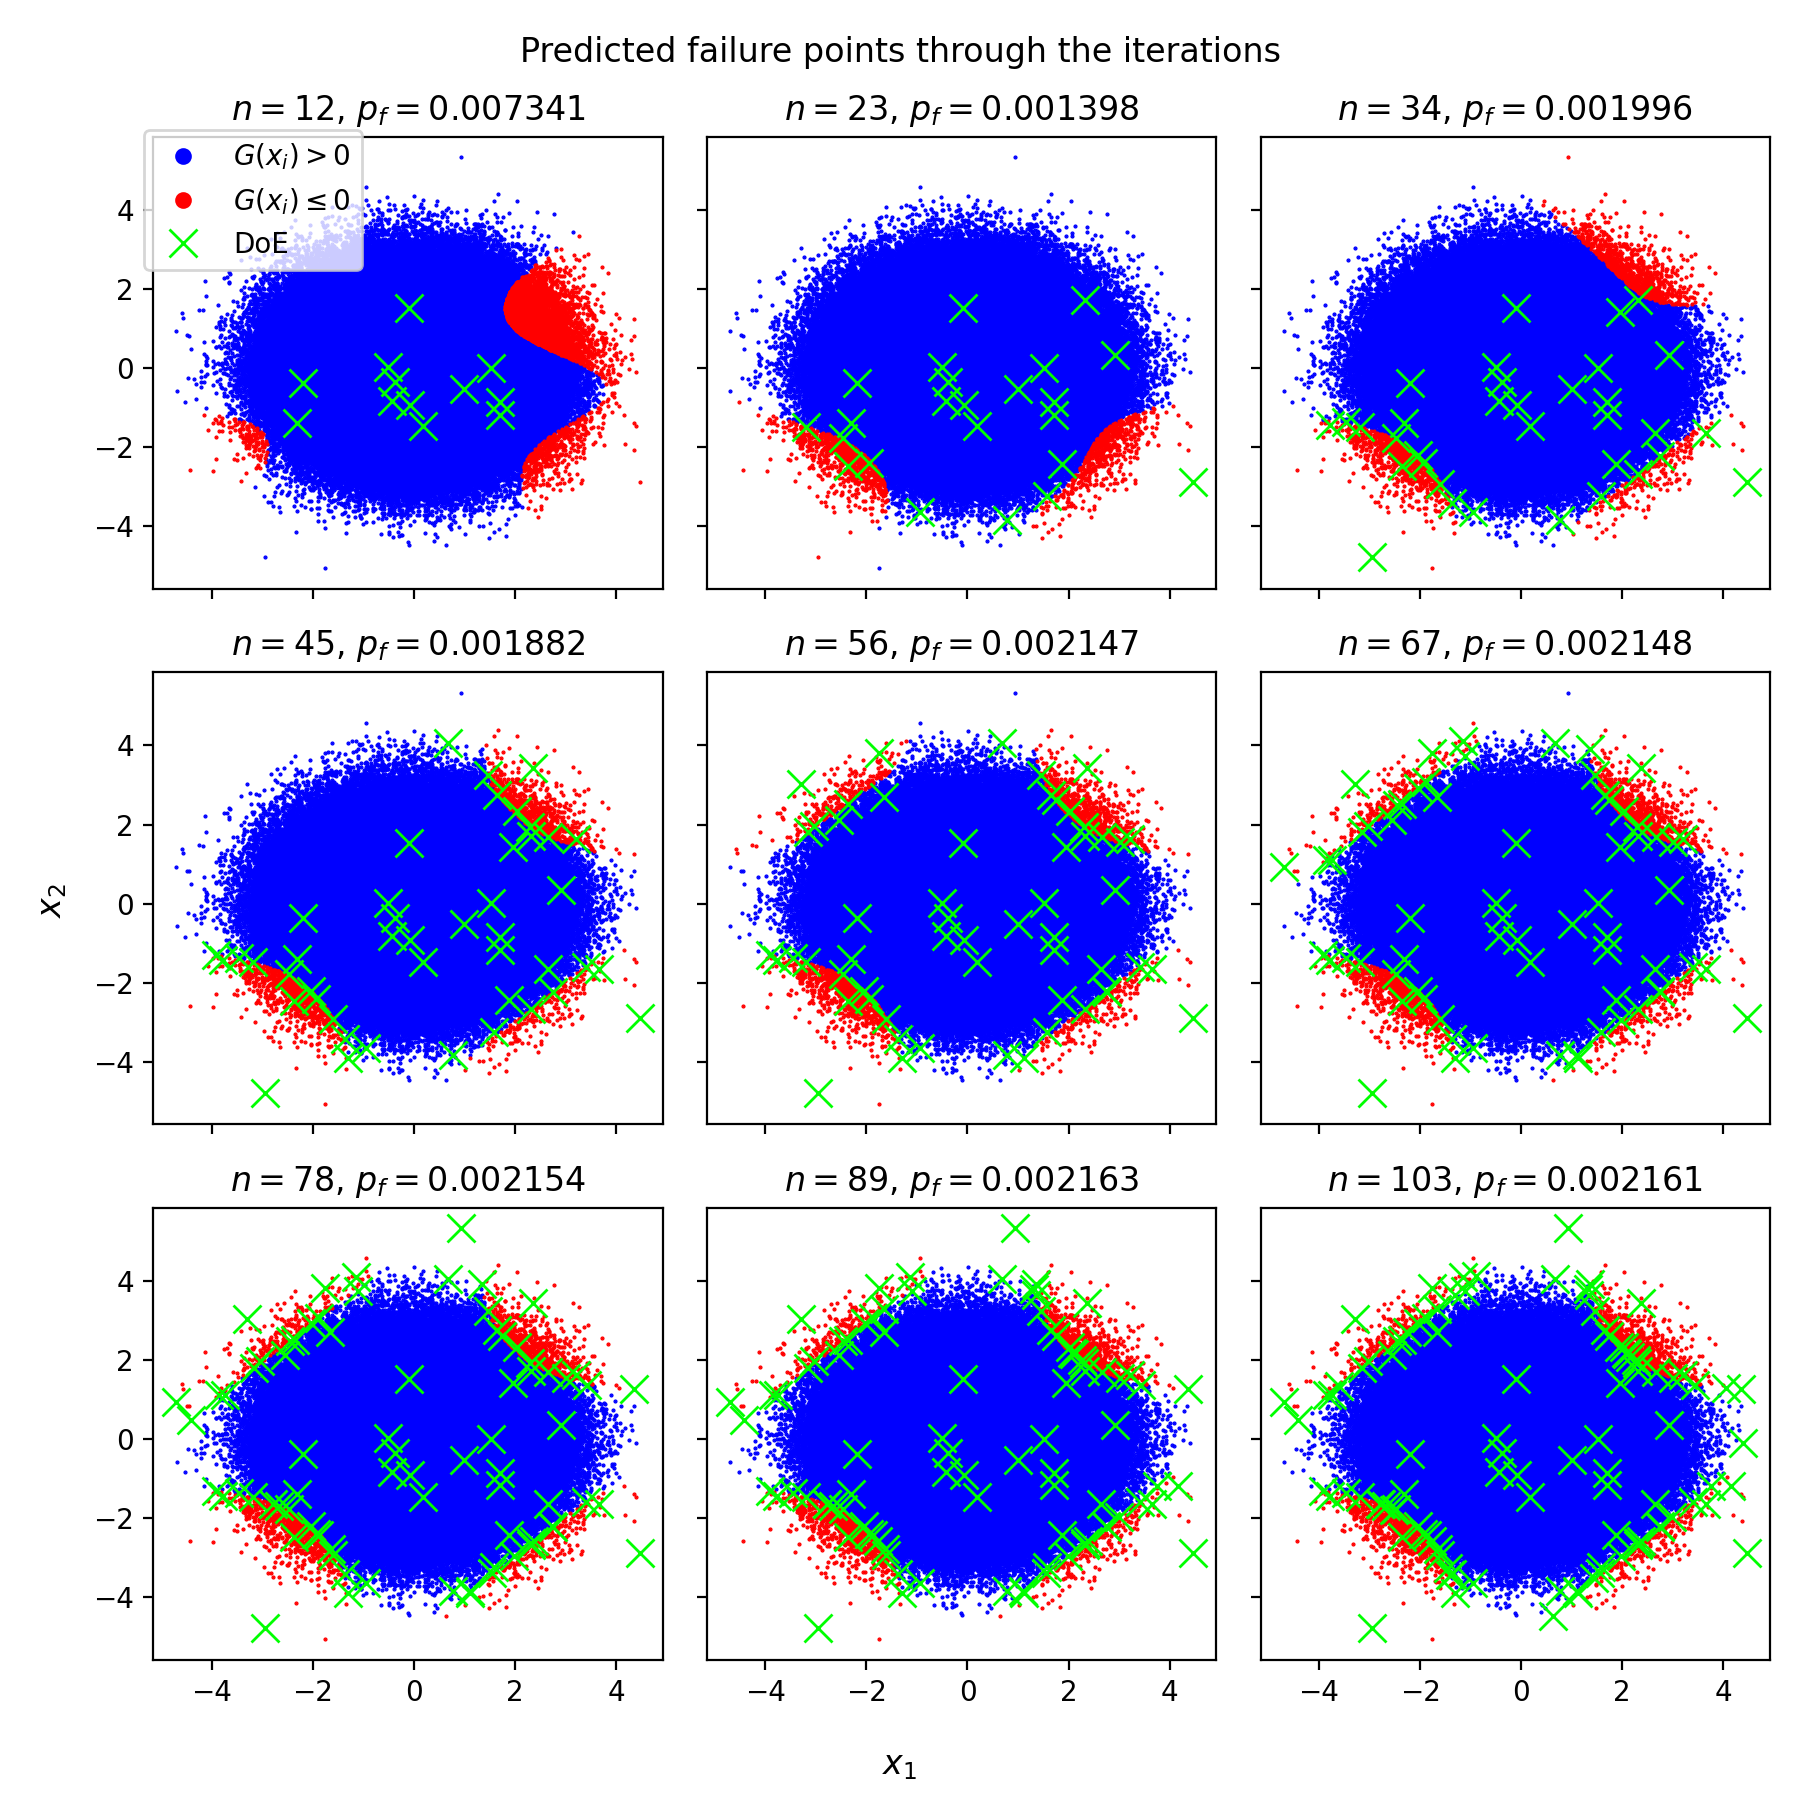
\includegraphics{iter_ex_2D_k7_U.png}
    \caption{Example 2 with $k=7$. Prediction made by AK-MCS+U at several stages.}
    \label{fig:ex2_iteru}
\end{figure*}

Figures  \ref{fig:ex2_k6} and \ref{fig:ex2_k7} display how the probability of failure
converges with each learning function, and how the selected points make the learning criteria
tend to the stopping conditions. In both cases there are similar behaviors. The 
EFF is proned to converge more consistently to the stopping condition. The function 
U usually gets a good estimation well before finishing. The function H
presents the most irregular results. A stricter stopping condition would be more appropiate
for this last learning function.

\begin{figure*}[h]
    \begin{subfigure}{.5\textwidth}
        \centering
        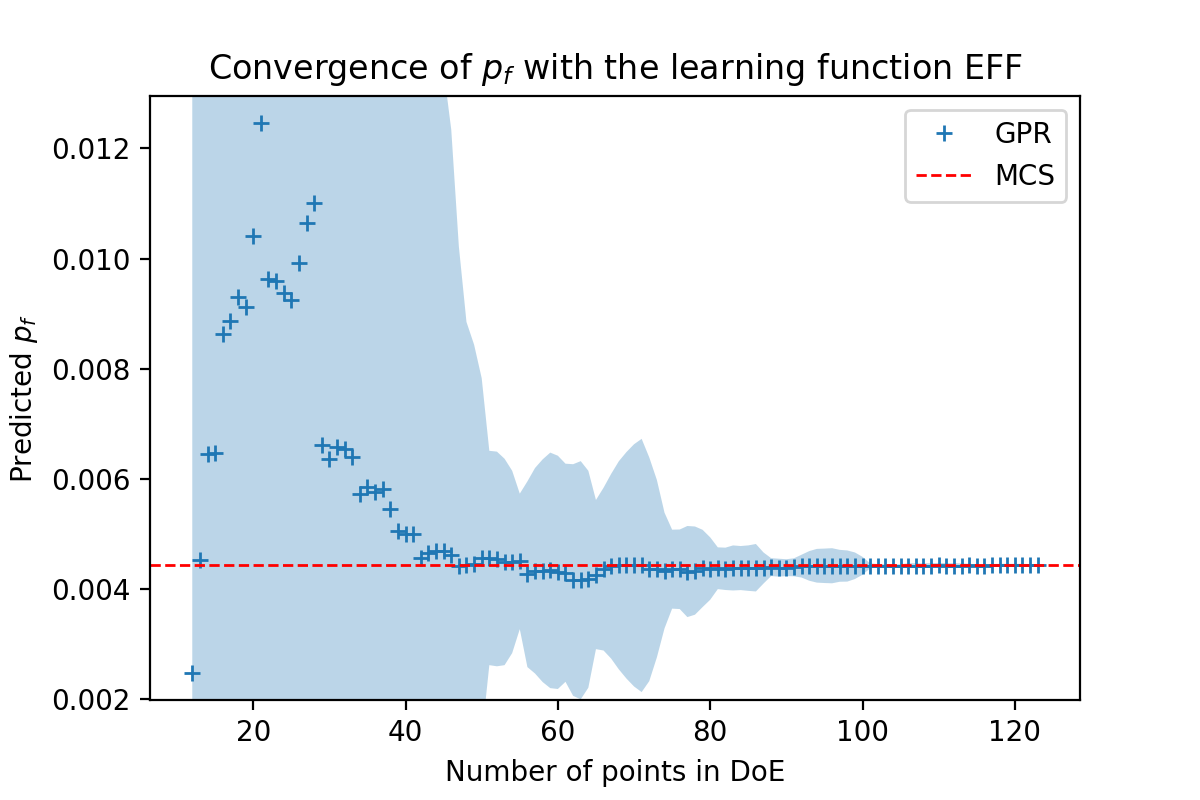
\includegraphics[width=\linewidth]{conv_ex_2D_k6_EFF.png}
      \end{subfigure}%
      \begin{subfigure}{.5\textwidth}
        \centering
        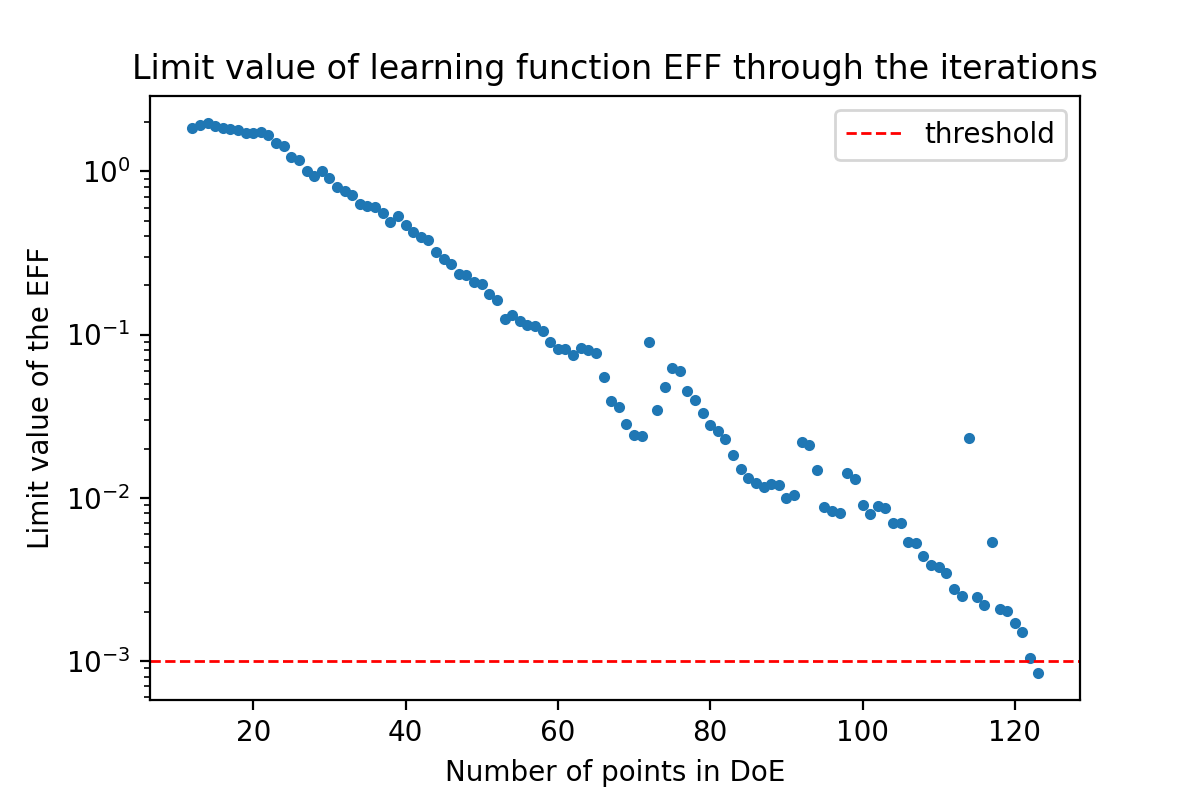
\includegraphics[width=\linewidth]{ex_2D_k6_EFF_lim_values.png}
      \end{subfigure}%
      \\
      \begin{subfigure}{.5\textwidth}
        \centering
        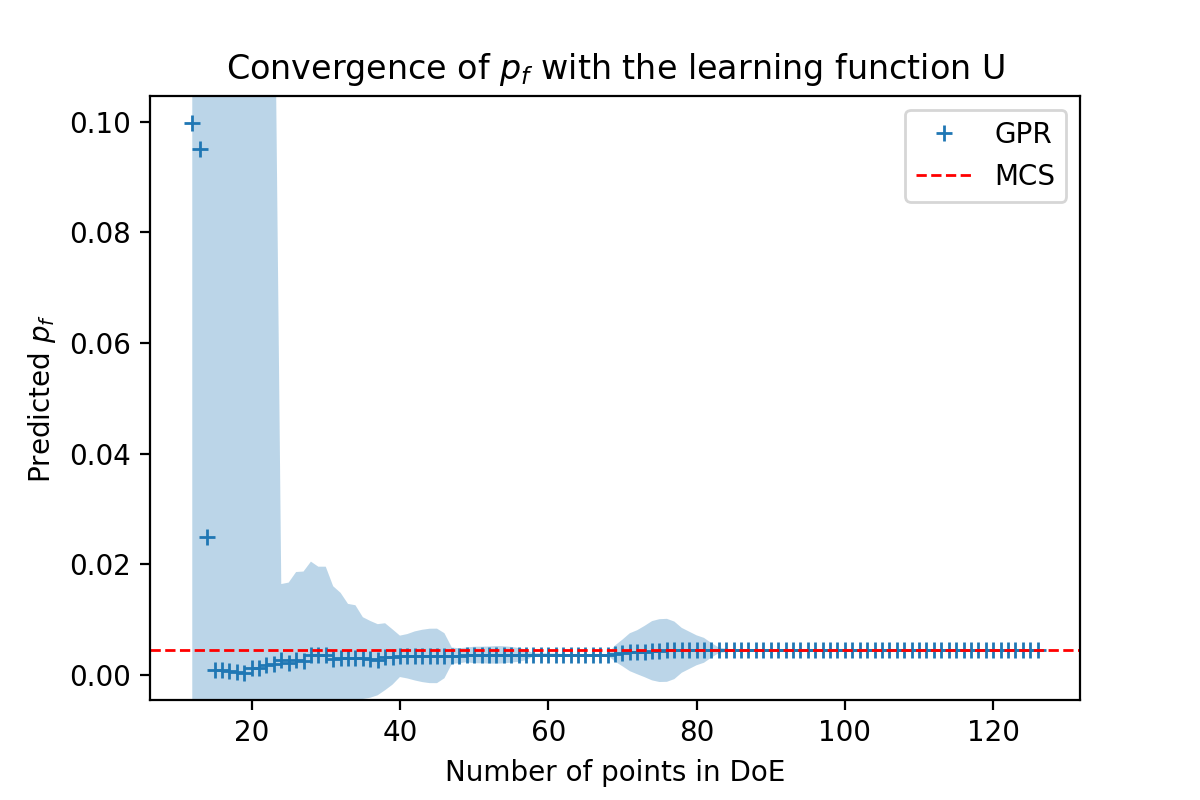
\includegraphics[width=\linewidth]{conv_ex_2D_k6_U.png}
      \end{subfigure}%
      \begin{subfigure}{.5\textwidth}
        \centering
        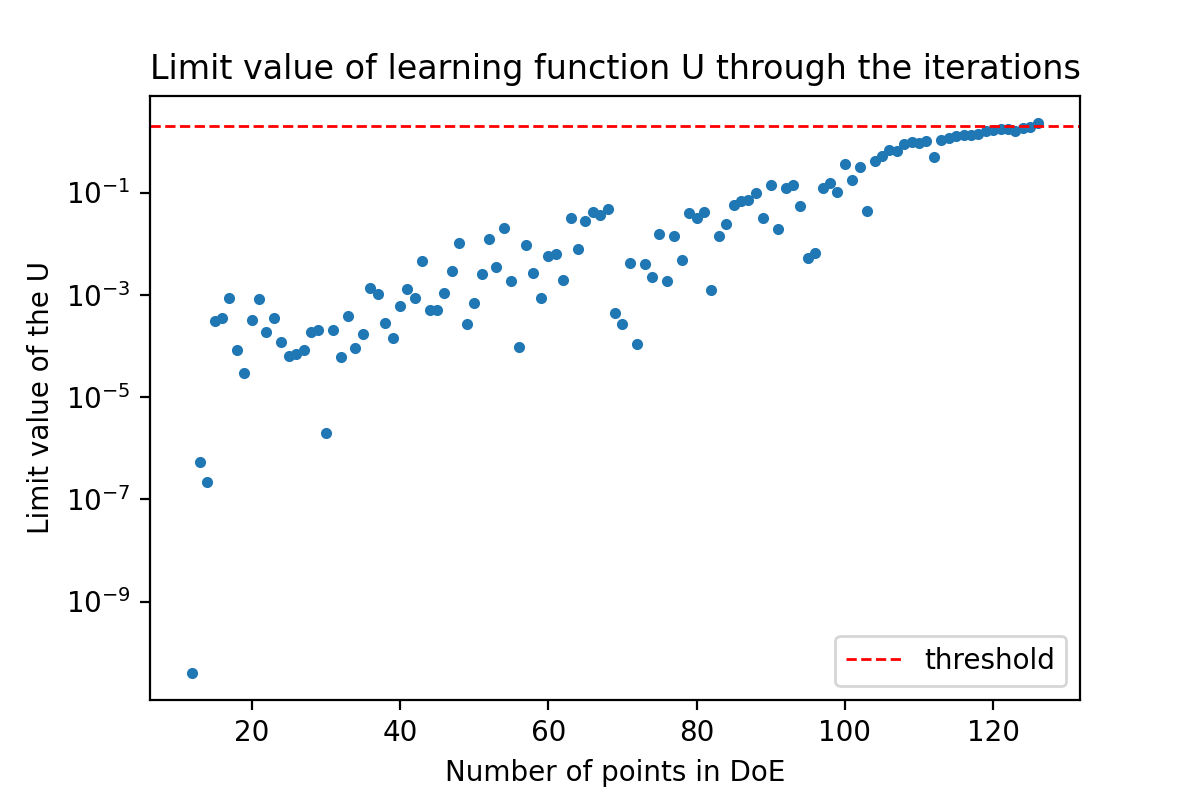
\includegraphics[width=\linewidth]{ex_2D_k6_U_lim_values.png}
      \end{subfigure}%
      \\    \begin{subfigure}{.5\textwidth}
        \centering
        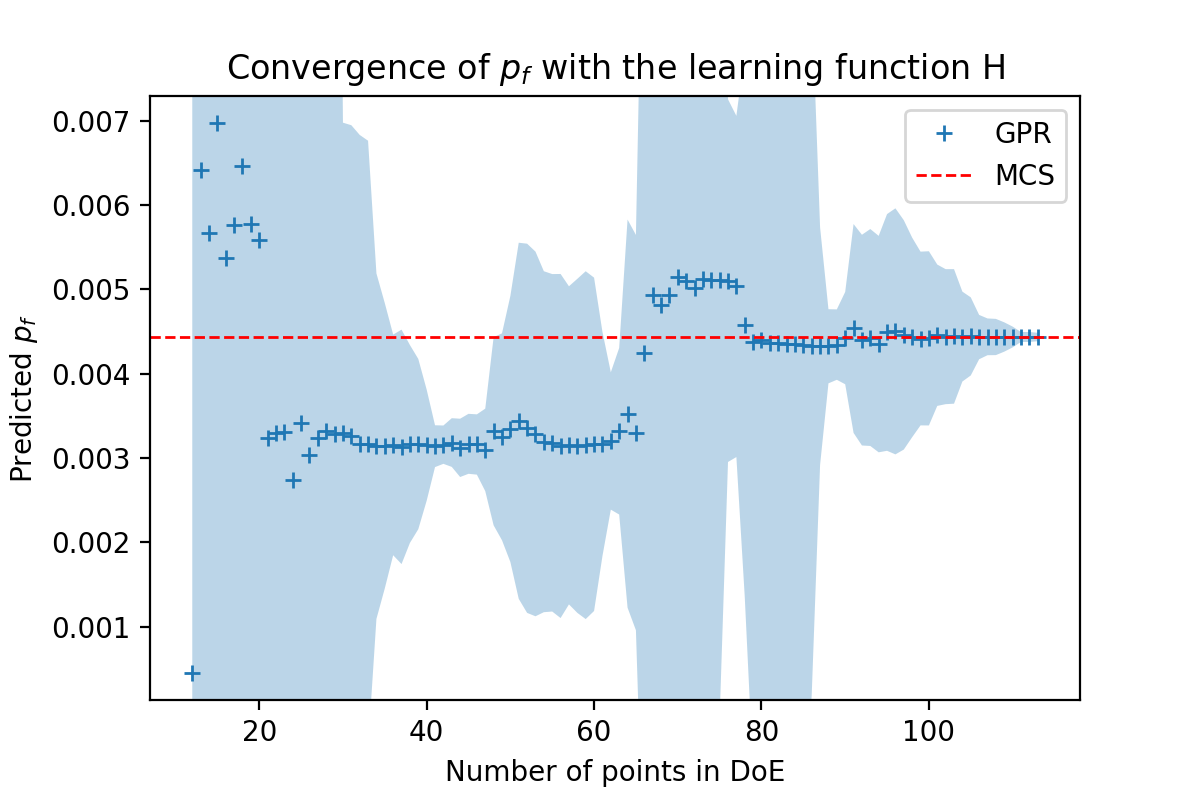
\includegraphics[width=\linewidth]{conv_ex_2D_k6_H.png}
      \end{subfigure}%
      \begin{subfigure}{.5\textwidth}
        \centering
        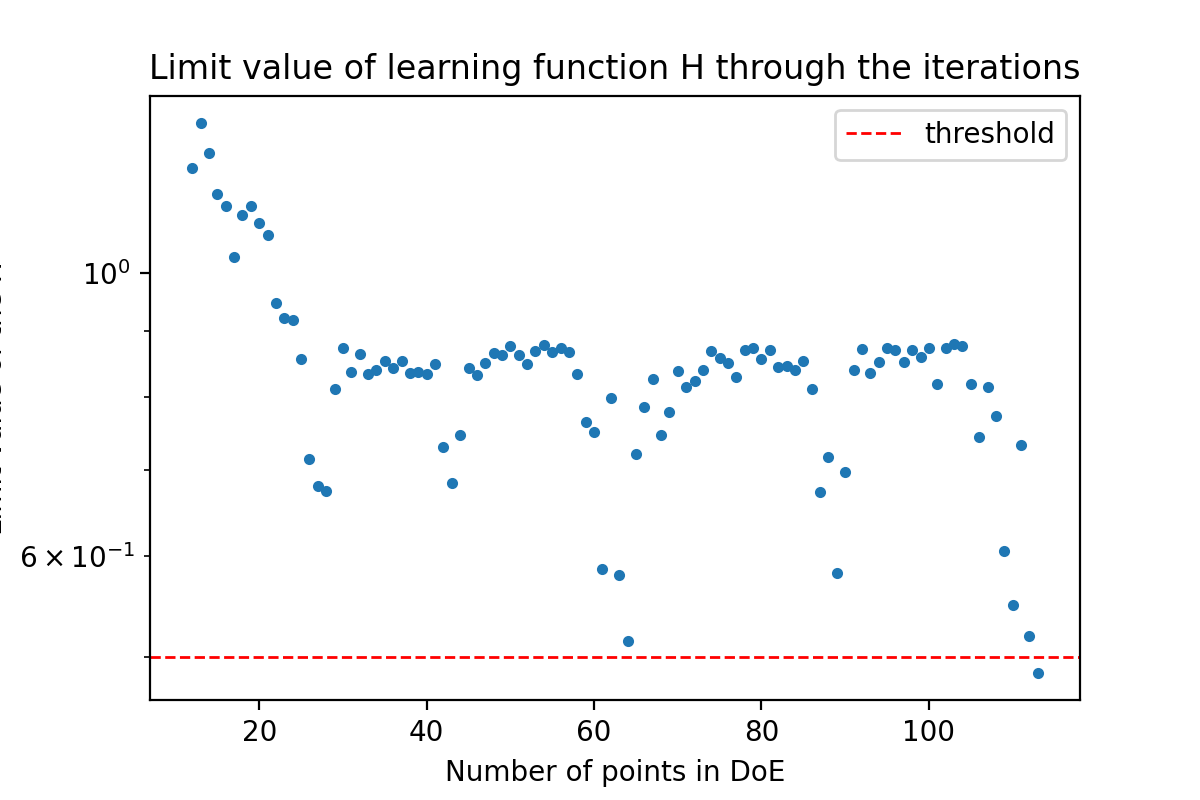
\includegraphics[width=\linewidth]{ex_2D_k6_H_lim_values.png}
      \end{subfigure}%
      \caption{Results of example 2 with $k=6$}
      \label{fig:ex2_k6}
\end{figure*}

\begin{figure*}[h]
    \begin{subfigure}{.5\textwidth}
        \centering
        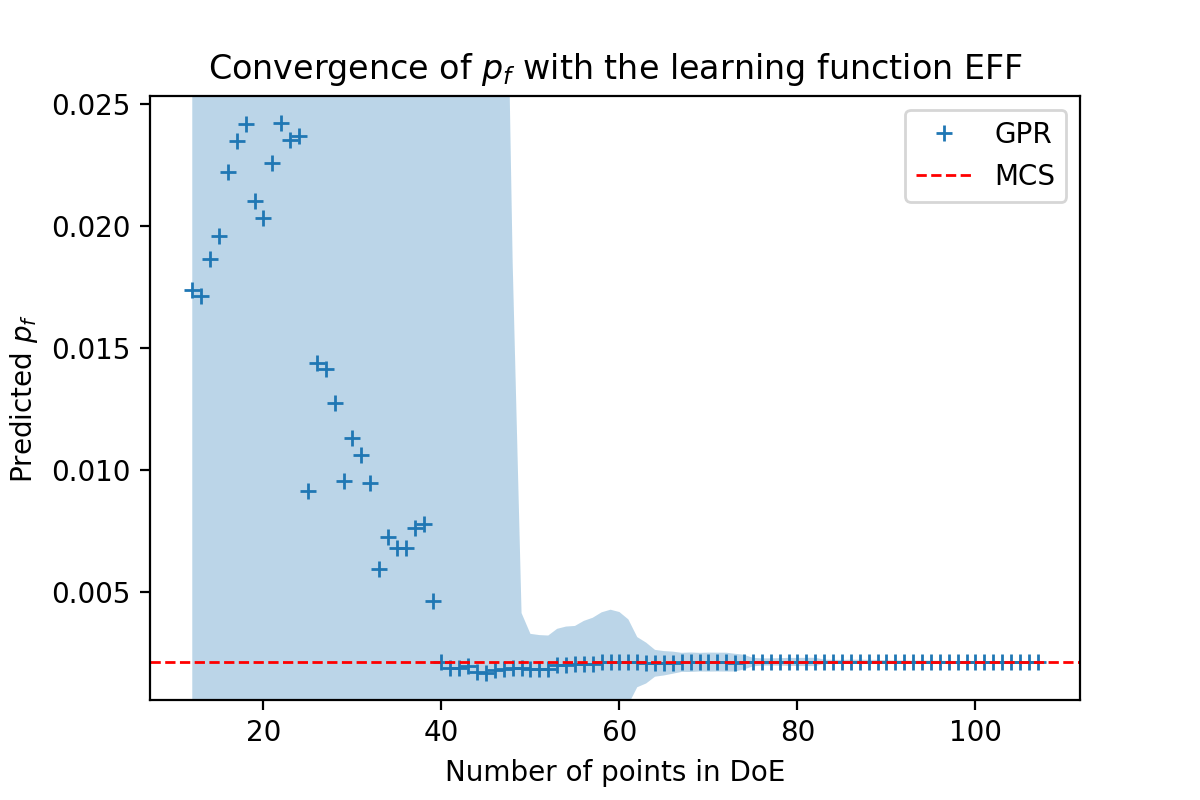
\includegraphics[width=\linewidth]{conv_ex_2D_k7_EFF.png}
      \end{subfigure}%
      \begin{subfigure}{.5\textwidth}
        \centering
        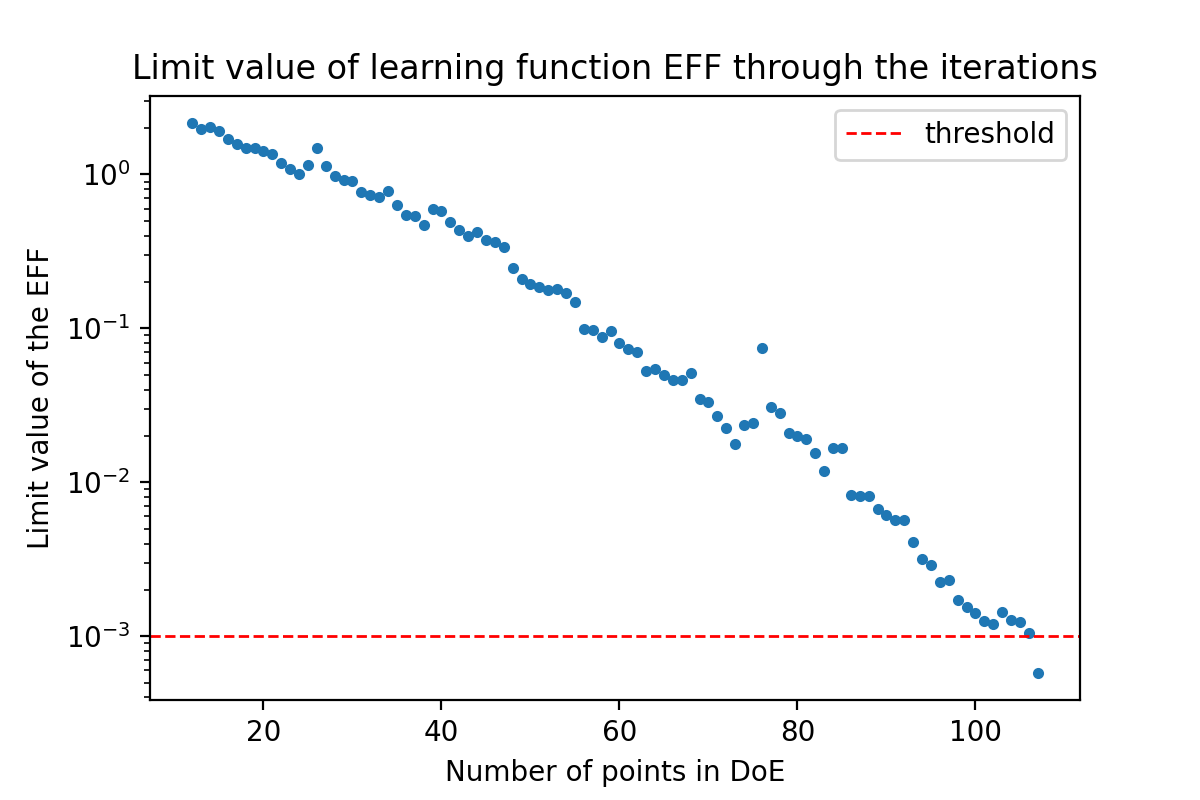
\includegraphics[width=\linewidth]{ex_2D_k7_EFF_lim_values.png}
      \end{subfigure}%
      \\
      \begin{subfigure}{.5\textwidth}
        \centering
        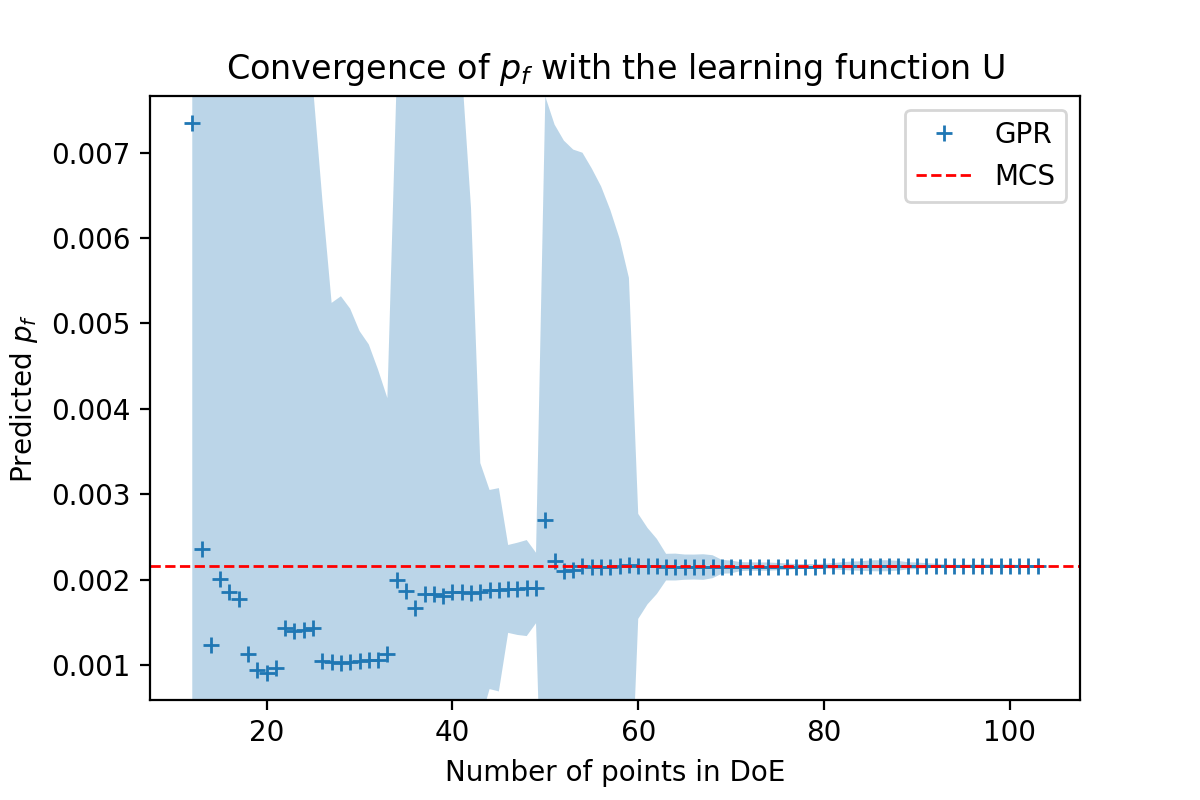
\includegraphics[width=\linewidth]{conv_ex_2D_k7_U.png}
      \end{subfigure}%
      \begin{subfigure}{.5\textwidth}
        \centering
        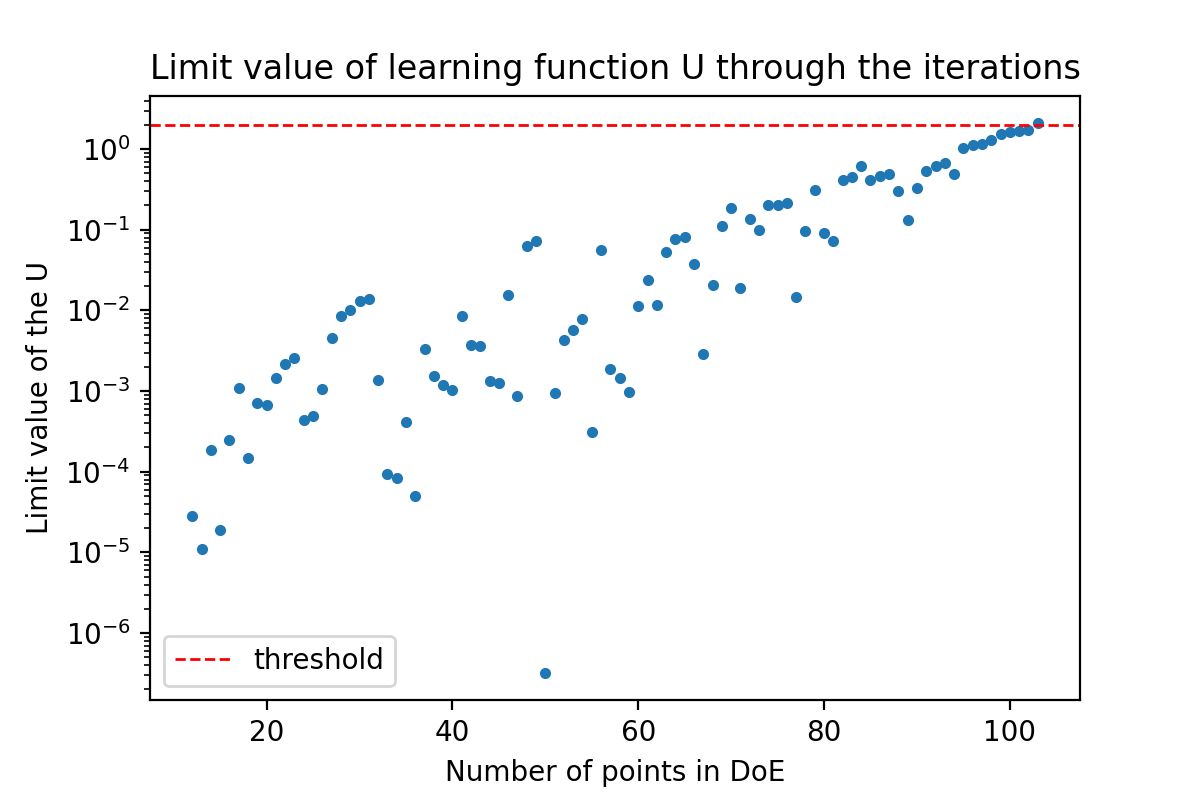
\includegraphics[width=\linewidth]{ex_2D_k7_U_lim_values.png}
      \end{subfigure}%
      \\    \begin{subfigure}{.5\textwidth}
        \centering
        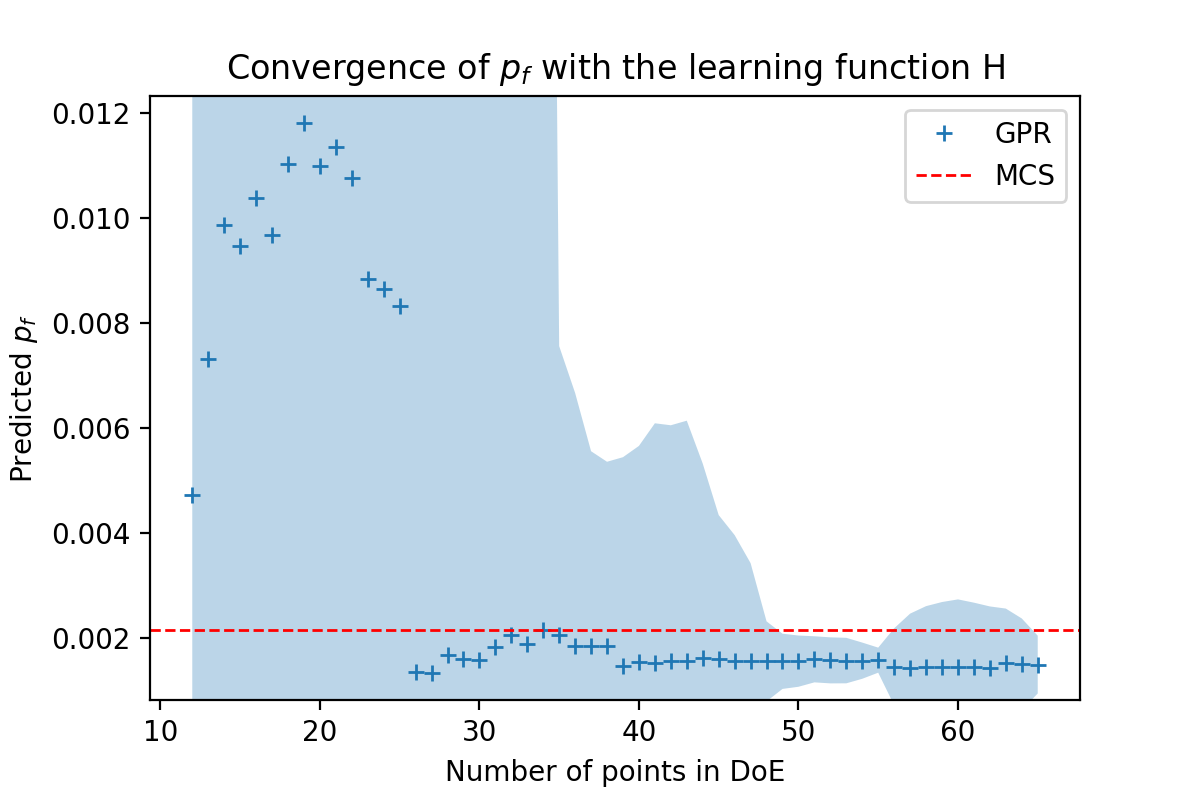
\includegraphics[width=\linewidth]{conv_ex_2D_k7_H.png}
      \end{subfigure}%
      \begin{subfigure}{.5\textwidth}
        \centering
        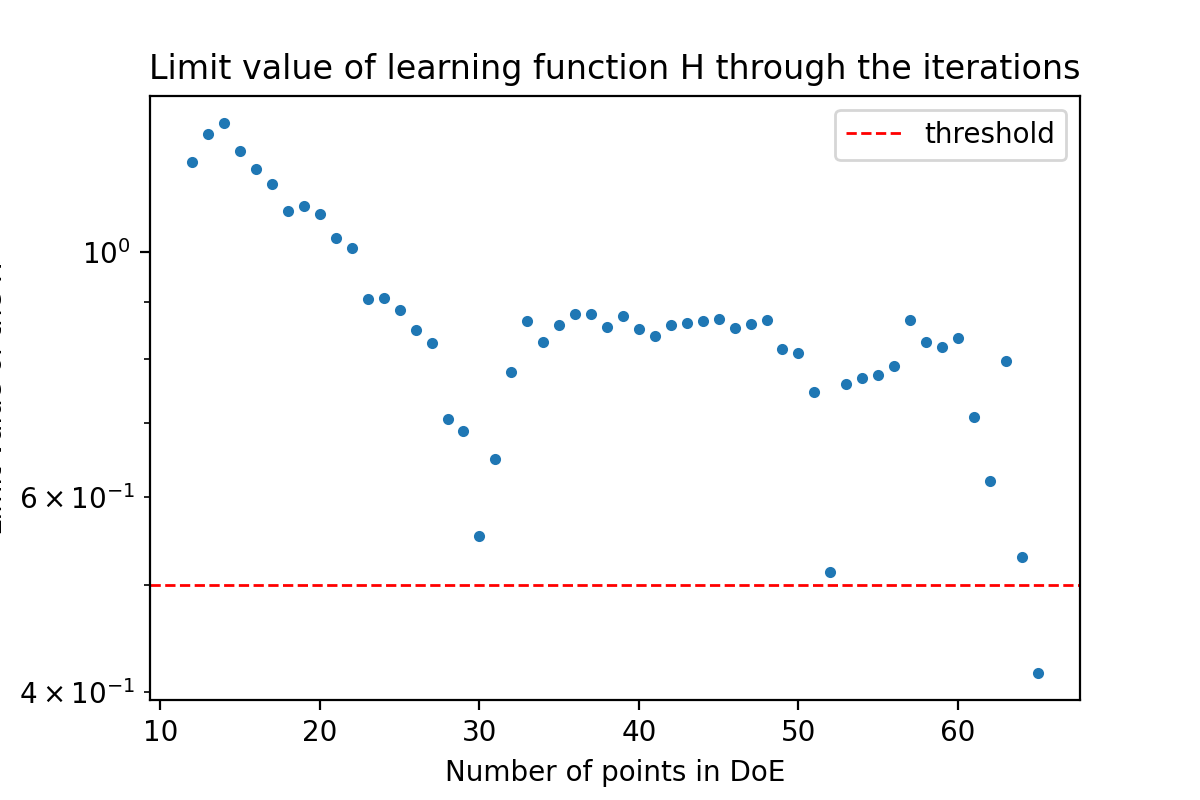
\includegraphics[width=\linewidth]{ex_2D_k7_H_lim_values.png}
      \end{subfigure}%
      \caption{Results of example 2 with $k=7$}
      \label{fig:ex2_k7}
\end{figure*}

\newpage
\subsection{Example 3}
The next example is a non-linear undamped single degree of freedom system, as the
one shown in figure \ref{fig:ex3}. The involved variables are listed in table \ref{tab:var_ex3}.

\begin{equation}
  G(\pmb{x}) = 3r - \left\lvert\frac{2F_i}{m\omega_0^2} \sin{\paren{\frac{\omega_0 t_1}{2}}} \right\rvert
\end{equation}
where $\omega_0 = \sqrt{\frac{c_1 + c_2}{m}}$

\begin{figure}[h]
    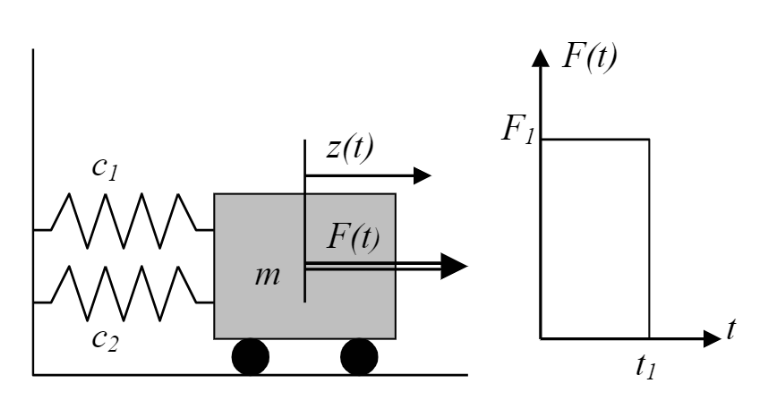
\includegraphics{ex_3.png}
    \caption{Example 3. Non-linear oscilator. Taken from \citep{Schu2005}}
    \label{fig:ex3}
\end{figure}

\begin{table}[h]
    \footnotesize%
    \begin{center}
    \begin{tabular}{cccc}
    \toprule
    Variable & P.D.F & Mean & Standard deviation \\
    \midrule
    $m$   & Normal & $1$ & $0.05$ \\
    $c_1$   & Normal & $1$ & $0.1$ \\
    $c_2$   & Normal & $0.1$ & $0.01$ \\
    $r$   & Normal & $0.5$ & $0.05$ \\
    $F_1$   & Normal & $1$ & $0.2$ \\
    $t_1$   & Normal & $1$ & $0.2$ \\
    \bottomrule
    \end{tabular}
    \end{center}
    \caption{Random variables of example 3}
    \label{tab:var_ex3}
\end{table}

Table \ref{tab:res_ex3} contains the obtained results. In contrast with the other
examples, in this case the function H performs quite well, obtaining the exact result, just
as the function U, but with some more calls to the performance function. \\

In figure \ref{fig:ex3_results} it is evident that the function EFF met its stopping
condition before converging to the solution, unlike the other two functions.

\begin{table}[h]
    \footnotesize
    \begin{center}
    \begin{tabular}{lclc}
    \toprule
    Method & $N_{call}$  & $\widehat{p_f}$ $(\text{C.O.V}_{\widehat{p_f}})$ &$\epsilon_{\widehat{p_f}}(\%)$  \\
    \midrule
    Monte Carlo   & \num[round-precision=1,round-mode=figures]{70000} & \num{0.027814}($2.23\%$) & - \\
    AK-MCS+U & $60$ & \num{0.027814} & $0$ \\
    AK-MCS+EFF & $43$ & \num{0.027671} & $0.51$ \\
    AK-MCS+H & $66$ & \num{0.027814} & $0$ \\
    \bottomrule
    \end{tabular}
    \end{center}
    \caption{Results of example 3}
    \label{tab:res_ex3}
\end{table}

\begin{figure*}[h]
    \begin{subfigure}{.5\textwidth}
        \centering
        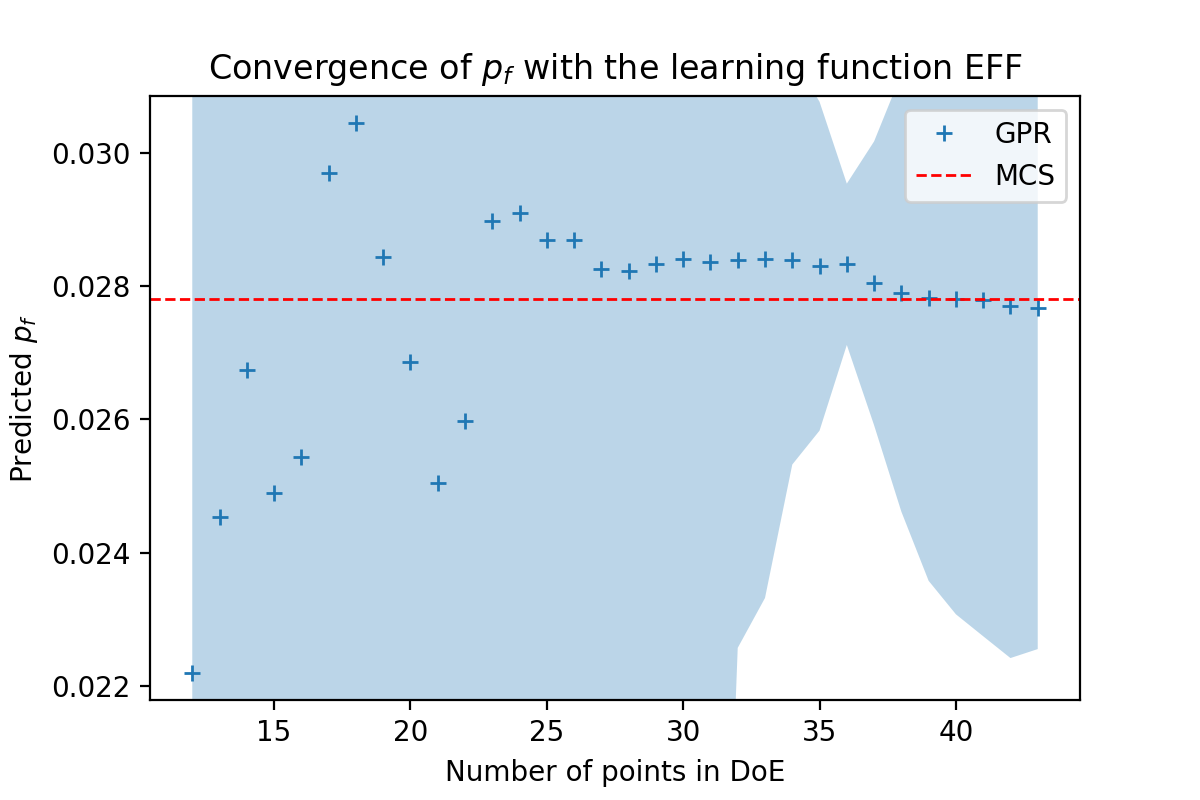
\includegraphics[width=\linewidth]{conv_ex_3_EFF.png}
      \end{subfigure}%
      \begin{subfigure}{.5\textwidth}
        \centering
        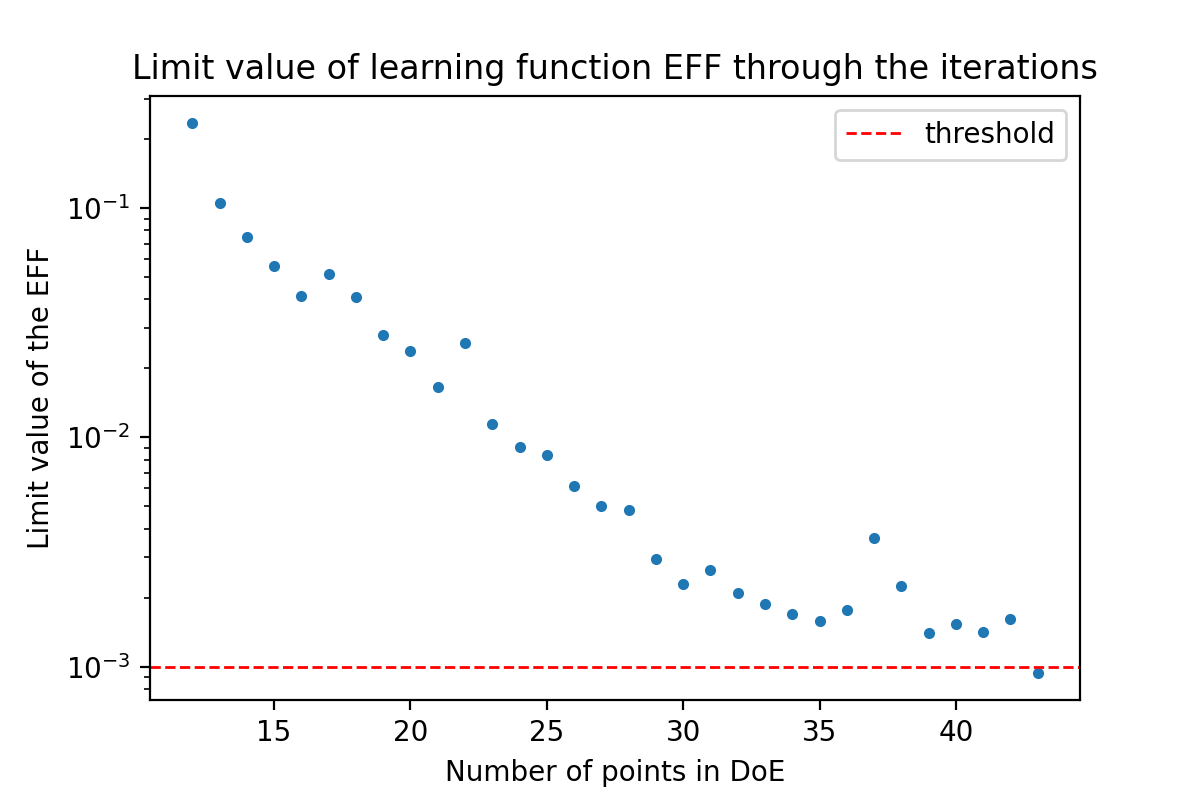
\includegraphics[width=\linewidth]{ex_3_EFF_lim_values.png}
      \end{subfigure}%
      \\
      \begin{subfigure}{.5\textwidth}
        \centering
        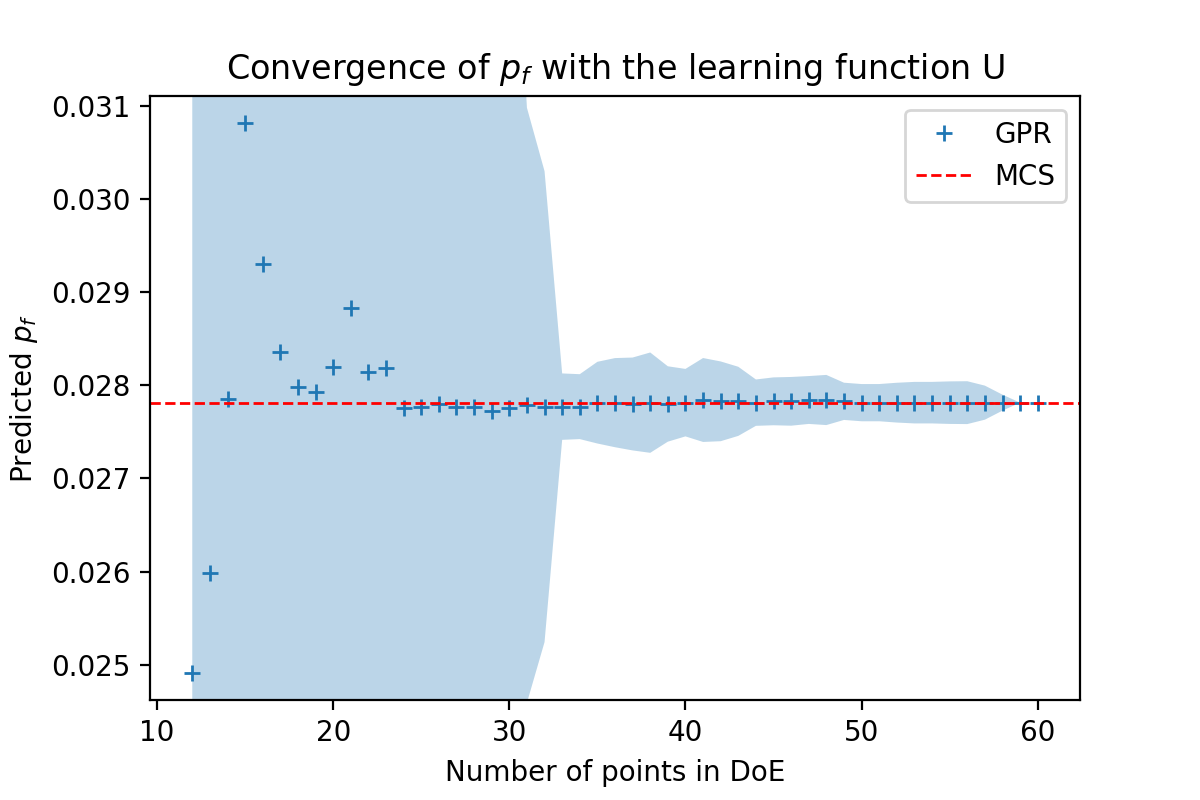
\includegraphics[width=\linewidth]{conv_ex_3_U.png}
      \end{subfigure}%
      \begin{subfigure}{.5\textwidth}
        \centering
        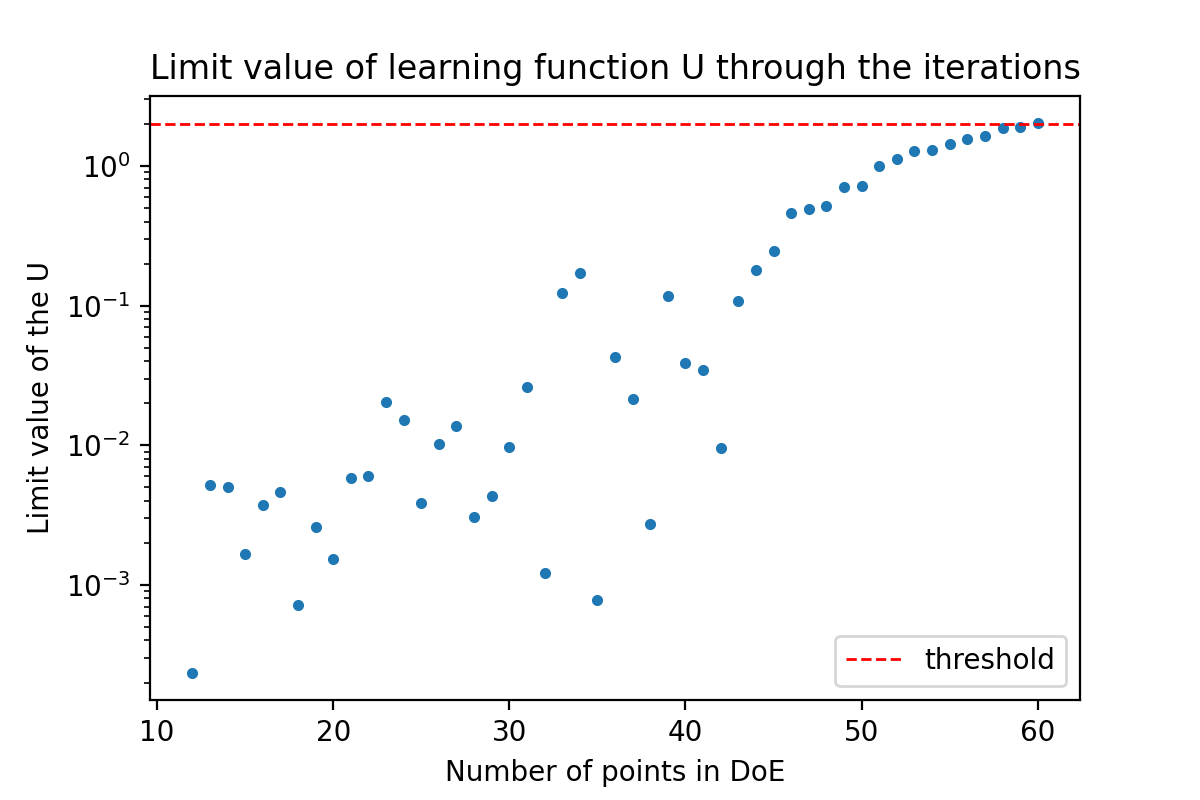
\includegraphics[width=\linewidth]{ex_3_U_lim_values.png}
      \end{subfigure}%
      \\    \begin{subfigure}{.5\textwidth}
        \centering
        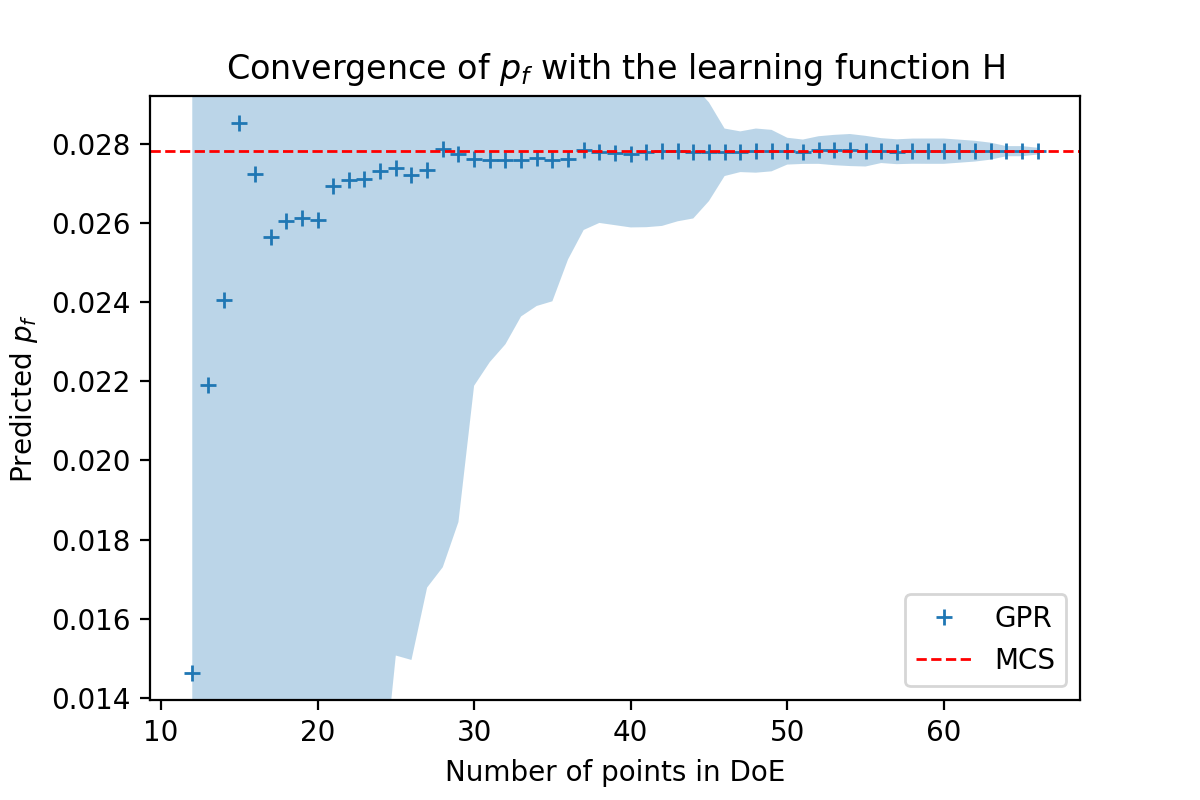
\includegraphics[width=\linewidth]{conv_ex_3_H.png}
      \end{subfigure}%
      \begin{subfigure}{.5\textwidth}
        \centering
        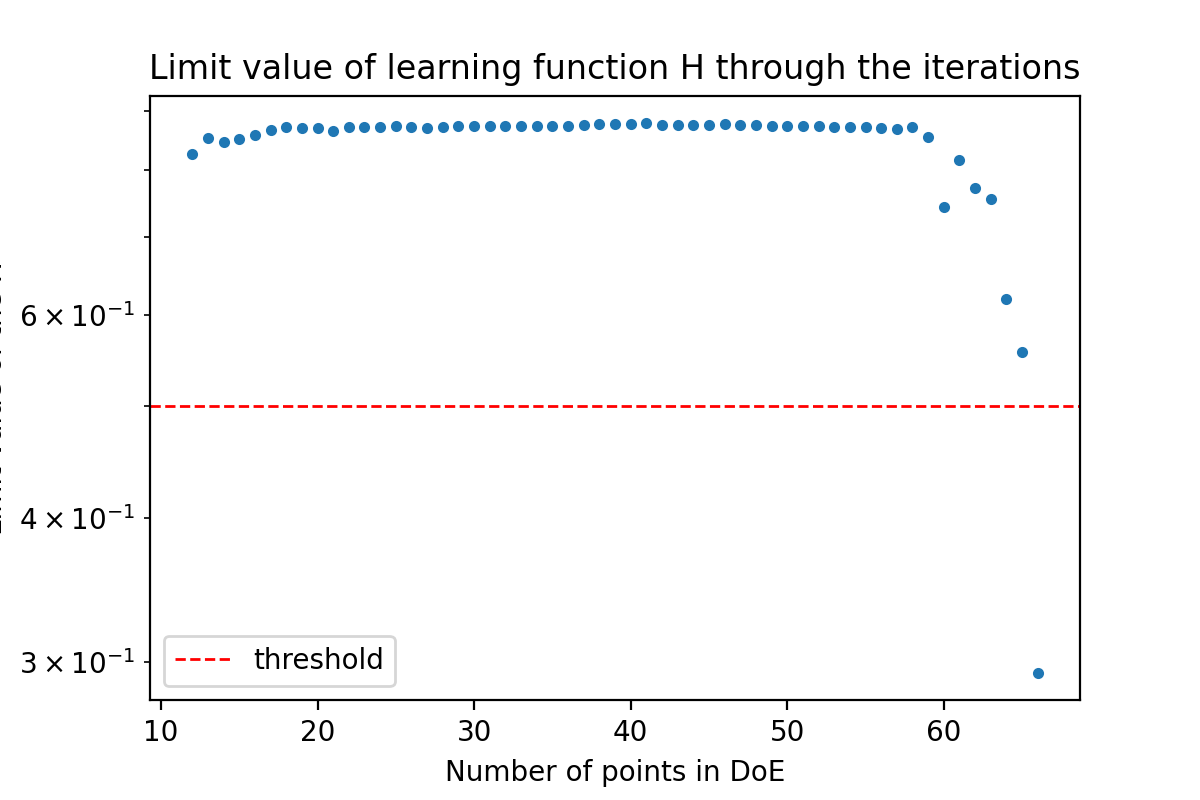
\includegraphics[width=\linewidth]{ex_3_H_lim_values.png}
      \end{subfigure}%
      \caption{Results of example 3}
      \label{fig:ex3_results}
\end{figure*}